	En la figura \ref{fig:infoAlumno} se puede observar un modelado de los datos que serán utilizados en el \refElem{Calmecac} para los almacenar la información de los alumnos del Instituto tal como :
	\begin{Citemize}
		\item Datos personales del alumno.
		\item Datos médicos del alumno.
		\item Datos deportivos del alumno.
		\item Datos académicos del alumno.
	\end{Citemize}

\begin{figure}[hbtp!]
	\begin{center}
	\fbox{\label{fig:infoAlumno}
		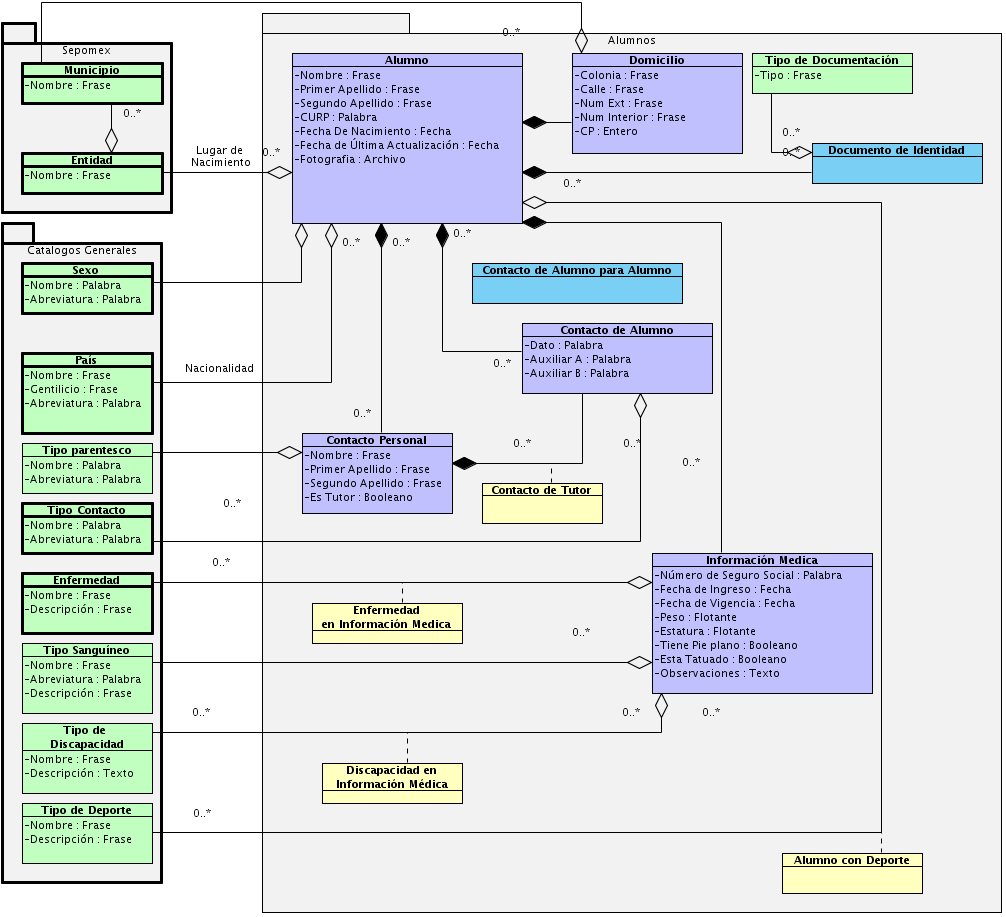
\includegraphics[width=\textwidth]{negocio/images/Estudiante_MDI}}
		\caption{Modelo de Información del Alumno}
	\end{center}
\end{figure}

\section{Alumno}

	En este paquete se encuentran todas las entidades y datos del Alumno de acuerdo a la toma de requerimientos hasta esta iteración del proyecto, muchas de las cuales son resultado de las relaciones entre el Alumno y los catálogos generales del CALMÉCAC.

\begin{cdtEntidad}[Un alumno es una persona inscrita en algún programa académico que se imparta en cualquier nivel educativo y modalidad educativa que ofrece el Instituto Politécnico Nacional.]{Alumno}{Alumno}
	\brAttr{nombre}{Nombre}{frase}{Representa la palabra o conjunto de palabras con las que se designan y se distinguen a una persona esta inscrita en algún programa académico impartido en el Instituto.}{\datOpcional}
	\brAttr{primerApellido}{Primer Apellido}{frase}{Representa la palabra o conjunto de palabras que sigue al nombre de pila de una persona y que se transmite de padres a hijos.}{\datOpcional}
	
	\brAttr{segundoApellido}{Segundo Apellido}{frase}{Representa la palabra o conjunto de palabras que sigue al primer apellido de una persona y que se transmite de padres a hijos.}{\datOpcional}
	
	\brAttr{CURP}{CURP}{palabra}{Representa la clave alfanumérica compuesta de 18 caracteres que permite identificar a un ciudadano residente de México. En el Instituto es otro de los mecanismos que ayudan a identificar a una persona que esta inscrito a algún programa académico impartido en el Instituto.}{\datOpcional}
	
	\brAttr{fechaDeNacimiento}{Fecha de Nacimiento}{fecha}{Es la fecha que, en el Acta de Nacimiento de una persona, establece el día en que nació.}{\datOpcional}
	
	\brAttr{fechaDeActualizacion}{Fecha de Actualización}{fecha}{Indica la fecha en la que en el sistema se llevo a cabo una modificación o actualización en los datos o relaciones de una persona con otras entidades.}{\datOpcional}
	
	\brAttr{fotografia}{Fotografía}{archivo}{Es el conjunto de datos almacenados dentro de una extensión especifican que contiene una imagen del rostro del Alumno. }{\datOpcional}
\end{cdtEntidad}

